\documentclass[11pt]{article}
\usepackage{latexsym}
\usepackage{caption2}
\usepackage{flafter}
\usepackage{graphicx}
\usepackage[sort,numbers]{natbib}
\setlength{\bibsep}{-0.5pt}
\usepackage{tcolorbox}
\newtcolorbox{mybox}{colback=grey!5!white,colframe=red!75!black}
\usepackage[]{setspace}
\usepackage{amsfonts}
\usepackage{amssymb,amsmath}
%\usepackage[table]{xcolor}
\usepackage[mathlines,displaymath]{lineno}
\usepackage[T1]{fontenc}
\usepackage[latin1]{inputenc}
\usepackage{anyfontsize}
\usepackage{lipsum}
\usepackage{etoolbox}
\usepackage{float}
\usepackage{wrapfig}
\usepackage[framemethod=tikz]{mdframed}

\usepackage{tcolorbox}
\newtcolorbox{mybox}{colback=white!140,colframe=white!75}

\makeatletter
\patchcmd{\@maketitle}{\begin{center}}{\begin{flushleft}}{}{}
\patchcmd{\@maketitle}{\begin{tabular}[t]{c}}{\begin{tabular}[t]{@{}l}}{}{}
\patchcmd{\@maketitle}{\end{center}}{\end{flushleft}}{}{}
\makeatother

\newcommand{\etal}{{et~al.{}}}
\newcommand{\ie}{{i.~e.{}}}
\newcommand{\eg}{{e.~g.{}}}
\newcommand{\viz}{{viz.{}}}
\newcommand{\etc}{{etc.{}}}
\newcommand{\apriori}{{a priori{}}}
\newcommand{\vv}{{vice versa{}}}
\newcommand{\cf}{{}}
\usepackage{titling}
\usepackage{color}
\newcommand{\carlos}[1]{\textcolor{red}{#1}}
\newcommand{\toedit}[1]{\textcolor{blue}{#1}}
\setlength{\droptitle}{-10em}% This is my set screw

\oddsidemargin 0.3cm 
\textwidth 18cm 
\textheight 19cm 

\begin{document}
\pagestyle{empty}

 \vspace{-1.25 in}
\section*{Part 2: Description of Work}
\section*{1. Summary}
We are in a massive human-driven biodiversity extinction with
uncertain consequences for Earth climate, life conditions and the
stability of Earth (Figure 1). This rapid global change put us in an
edge to take in science the risks to reduce the uncertainty related to
the consequences of feedbacks between the Earth system and
biodiversity (Figure 2). The rapid decline of biological diversity
urges efforts from the scientific community to characterize and to
identify key players: Biodiversity is sustained by processes acting
across biological (i.e., from genes to traits and ecological
networks). Yet, the fussion of heterogeneous data spanning different
biological levels, taxa and ecosystems to decipher the
interdependencies among biological levels and how such
interdependences alter biodiversity response to rapid global change is
still not in place. This project will develop a deep learning
biodiversity platform based on processes to leverage data collected
from several sources to map future scenarios of biodiversity decline
in interdependent biological networks.
\subsection*{Statements of the goals}
Our main goal is to pursue how interdependent biological levels affect
biodiversity dynamics and its decline. Biodiversity research has been
sistematically studied at one biological level. While splitting
disciplines in many biological, temporal and spatial scales have
produced an immense gain in detailed knowledge at each of the levels
and scales studied, it might be insufficent to understand the
consequences of biodiversity dynamics when feedbacks between
biological levels occur (Figures 1 and 2). We propose to study
data-driven patterns within and between biological levels to decipher
the role of interdependencies for the maintenance of
biodiversity. Fussioning modern data analytics and theory in
biodiversity research would help to contrast process-based scenarios
of biodiversity decline with and without considering interdependences
across biological levels (Figure 2).
\subsection*{Milestones}
i) {\bf Deep process-based learning platform for biodiversity
  research}: We will explore deep-learning networks to contrast
patterns of biodiversity dynamics with and without feedbacks within and between the networks (Box 1 and Box 2).\\
ii) {\bf Visualization tools}: We will communicate in public
exhibitions the core patterns and processes governing interdependent
networks across biological levels and its impact on biodiversity
dynamics and current decline rates.
\subsection*{Significance of the project for data science}
We will bring deep process-based learning networks to biodiversity
research as a fundamental and applied tool to unfold the role of the
interdependencies among biological levels for understanding
biodiversity dynamics. We will be communicating in a permanent public
exhibition the importance of merging data science and biodiversity
research across biological levels for predicting future response
scenarios to rapid global change.  \vspace{-1.25 in}
\begin{mybox}
  \begin{center}
       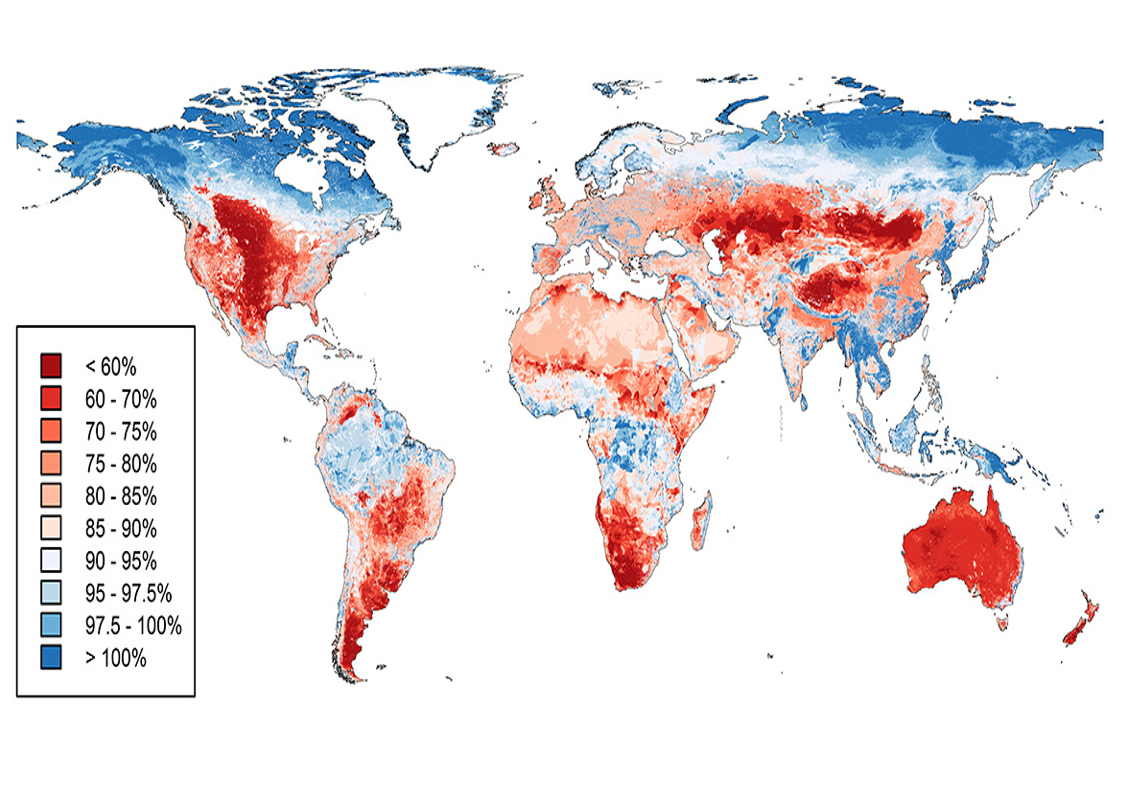
\includegraphics[width=0.6\textwidth]{Figure1.png}
     \end{center}
             \vspace{-0.45 in}

     \caption{{\small {\bf Figure 1: Biodiversity is declining globally at unprecedented
         rates}. Map showing the remaining populations of native
       species across many taxa as a percentage of their original
       populations. Blue areas are within proposed safe limits, and
       red areas are beyond these limits \citep{Newboldetal:2016}}}
   \vspace{-0.75 in}
     
\begin{center}
     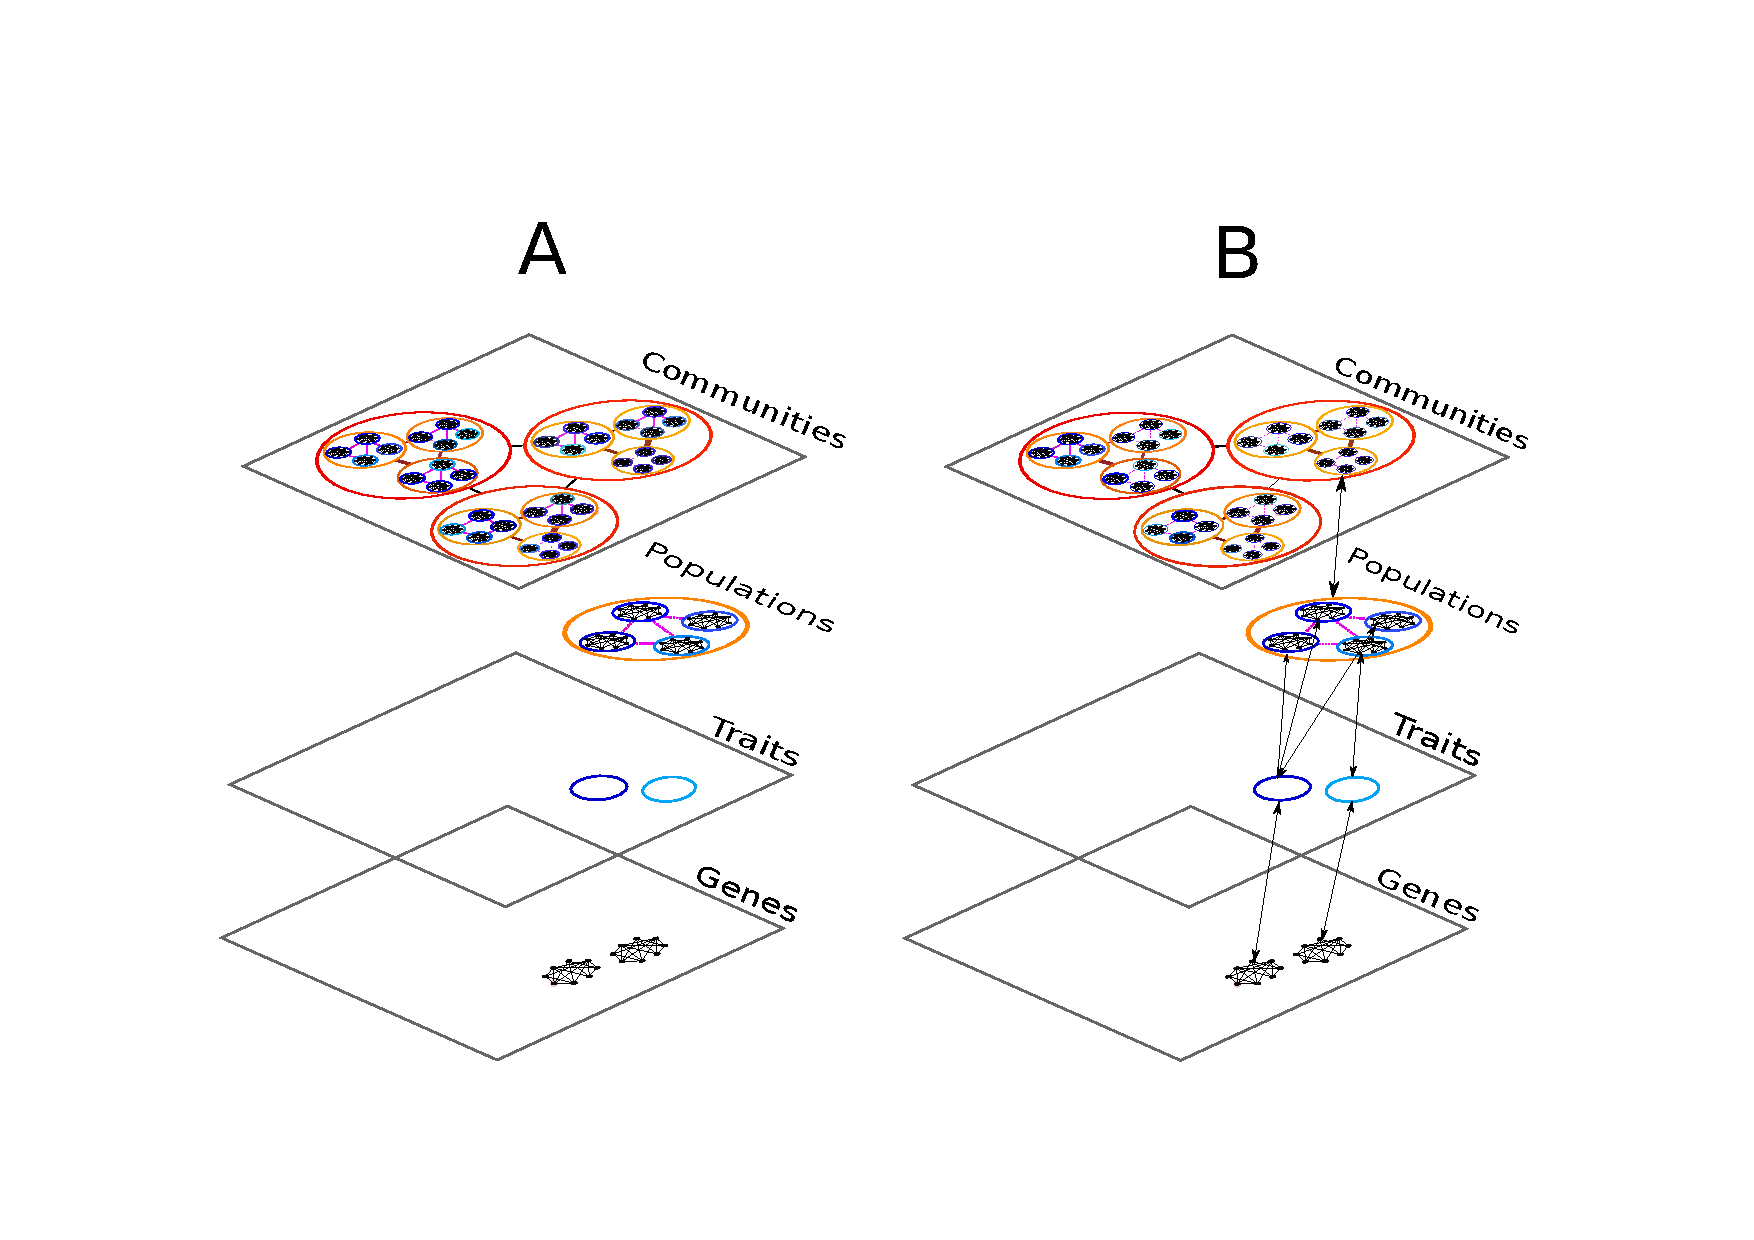
\includegraphics[width=0.8\textwidth]{Figure2.pdf}
   \end{center}
        \vspace{-0.65 in}
        \caption{{\small {\bf Figure 2: Biodiversity is sustained by
              processes acting across biological levels.} Yet,
            inferring interdependencies among levels to predict the
            consequences of biodiversity decline remains poorly
            studied. A) Biodiversity has been studied mostly
            considering independent levels: Genes, traits and
            populations to communities and ecological networks each
            are defined at one level without exploring the
            interdependencies. B) Biodiversity represented as
            interdependent levels accounting for feedbacks among
            genes, traits, populations and communities. It remains
            unknown which of these two scenarios more accurately
            predict current trends in biodiversity decline and its
            consequences for Earth climate, life conditions and the
            stability of Earth.}}
\end{mybox}



\newpage
\section*{2. Background and Significance to Data Science}%Background and significance to Data Science
The study of interactions, both within and across biological scales,
is central to the ongoing synthesis of biodiversity
\citep{Darwin:1964,Futuyma&Slatkin:1983,Thompson:2013}. Ecologists,
for example, have argued for empirical patterns of positive
\citep{MacArthur:1955}, negative \citep{May:1973} and
non-relationships \citep{Jacquetetal:2016} between the number of links
and the stability of food webs (i.e., the number of links usually
defined as the complexity of the food web). This debate is rooted in
the mechanisms driving ecological interactions accounting for
interactions among species
\citep{May:1973,dunne2005modeling,Thebault&Fontaine:2010,Allesina&Tang:2012,Johnsonetal:2014,Mougi&Kondoh:2016,Graveletal:2016}.

Analogously, evolutionary biologists have puzzled over the
relationships between the complexity of gene interactions and the
stability of phenotypes tha drive ecological interactions
\citep{Alberch:1991,Arnold:1992,Debat&David:2001,Wagner:2005}. Quantitative
genetics theory predicts that most genetic variance in populations is
additive \citep{Hilletal:2008}, and yet accounting for nonlinear gene
interactions can improve predictions about the distribution and
evolution of traits \citep{Forsbergetal:2017}. Experiments are also
increasingly showing that gene interactions are common and that
additivity can be an emergent property of underlying genetic
interaction networks
\citep{Stearns:2010,EyreWalker:2010,Wagner&Zhang:2011,Mackay:2014,North&Beaumont:2015,Pavlicevetal:2015}. Although
the relationship between complexity and stability has been explored
within biological levels, such as either genes, traits, populations or
food webs, the interdependencies among levels have received less
attention. Therefore, inferring interdependencies among biological
levels to predict their role in biodiversity maintenance remains
poorly studied
\citep{Whithametal:2006,Loeuille:2010,Fontaineetal:2011,Melianetal:2018}
(Figure 2).

Most methods in AI and Biodiversity research have been considered as
distinct fields. However, the current scientific ecosystem is at the
stage where merging methods from distinct fields is radically
transforming the discipline boundaries, the reproducibility of science
and our predicting-understanding power to build and test theories
\citep{Reichsteinetal:2019}. Recent approaches in ecology and
evolution have introduced deep learning methods for labelled data,
from which selection modes and demographic history can be jointly
inferred \citep{Sheehanetal:2016}. Yet, many of the recent approaches
applying deep learning methods in biodiversity have mostly focused at
one level of biological organization. While this might produce
additional gain in detailed knowledge at each level, it remains
unknown how many layers are needed for predicting and understanding
biodiversity patterns. The one-level and one-scale approach might be
insufficent to understand the consequences of biodiversity decline.

To gain predictive and understanding power in biodiversity research we
would need to develop deep process-based learning models accounting
for many layers and the topology of the interactions within and
between the layers
\citep{Whithametal:2006,Loeuille:2010,Fontaineetal:2011,Melianetal:2018}. Many
methods from data science and biological systems share fundamental
properties, but the full potential of these shared properties have not
been sufficiently explored \citep{Schmidhuber:2015}. Biological
systems are composed by many layers (Figure 2), and they can contain
interdependent hierarchies and feedbacks with interacting learning
entities within and also between the layers. Therefore, exploring deep
learning networks topologies accounting for feedbacks within and
between layers is a first step towards understanding biodiversity
dynamics using deep process-based learning networks (Box 2).


\section*{3. Scientific Goals and Objectives}
Our goal is to study data-driven patterns within and between
biological levels to decipher the role of interdependencies in
maintaining biodiversity (Box 1 and 2). We will combine our own source
data with other databases to develop deep process-based learning
networks in biodiversity research. We will contrast two scenarios: An
scenario without feedbacks within and between the biological levels
and a second scenario accounting for feedbacks within and between
layers to decipher the role of interdependencies across biological
levels for biodiversity maintenance (Box 2). These two scenarios will
be contrasted for a series of biodiversity patterns, mostly related to
biodiversity maintenance and decline rates.

\section*{4. Research Plan}

\section*{4.1 General description of the scientific approach}
Our research plan is described in the following two boxes: Box 1
highlights the inference of our source empirical data to decipher
patterns across biological levels. Box 2 describes deep process-based
learning networks in biodiversity research.

\section*{4.2 Data sources}
The following are our source datasets:\\
\begin{itemize}
\item {\bf Projet Lac database}\\
\\
This is a dataset containing Fish communities from the majority of
lakes of Switzerland\\
(https://www.eawag.ch/en/department/fishec/projects/projet-lac/). The
database contains approx. 60k fish individuals, 40k morphometrics and
8k sampling actions each containing spatial coordinates, morphological
traits, species abundances, habitats and DNA data.
\\
\item {\bf Whitefish community database}\\
\\
Whitefish community from the majority of lakes of North Alps.  The
database contains more than 2k fish individuals. Sampling locations,
morphological, ecological and microsatellite data is available in the
Dryad database (https://doi.org/10.5061/dryad.k183ft7).
\\
\item {\bf Threespine Stickleback database}\\
\\
The Threespine stickleback fish database contains genetic, isotope,
diet, morphometric, ecological and spatial data for around 1k
individuals (Figure 3).
\end{itemize}

\begin{comment}
Hosting these datasets in the SDSC platform might allow us to:
\begin{itemize}
\item Featuring animations of the Fish collection part of the FishEc database in a future
permanent exhibition hosted by the Natural History Museum in Bern. The animations will
hightlight the interactions from genes to landscapes integrating genetic, phenotypic,
ecological and spatial data (see M1 and M2 below). Please check
https://www.nmbe.ch/de/unser-angebot/unser-angebot/fuer-forschende/wirbeltiere
section Ichthyologie with Projet Lac being one of the projects contributing the most to
the current FishEc database and https://www.nmbe.ch/de/museum/aktuelles/monster-im-
saft for the status of this permanent exhibition.
\item Inferring patterns of interdependence throughout new uploads of source data (M3 and
Box 1).
\item Analyzing process-based models to explore biodiversity dynamics scenarios with the
aim to infer the processes that best reproduce the empirical patterns observed in the
databases (M4 and Box 2).
\end{comment}

\begin{mybox}\begin{singlespace}
{\bf{Box 1. Inferring patterns of interdependence in model systems}}\\
\begin{small} 
  There are a few model systems with multidimensional data (section
  4.2 Data Sources for a non-exhaustive list). We have performed a
  preliminary analysis of the Threespine Stickleback database
  containing genetic (QTL mapping), phenotypic (morphological),
  isotope, trophic (diets) and spatial (habitat) data for around 1k
  individuals. Our analysis show a normally distributed pairwise
  correlation pattern indicating a high degree of no correlations in
  the data (Figure 3a). A large cluster contains a high proportion of
  the individuals, but many small clusters and isolated individuals
  also occur (not shown) indicating high dimensionality of the data
  (Figure 3b: color indicates different clusters each containing
  similar individuals). We will explore an methods to infer the
  interdependence among genetic, phenotypic, isotope, trophic and the
  spatial dimensions of our source data
  \citep{Schmidhuber:2015,Bianconi:2018} (Figure 3c shows the target
  for this analysis with each level containing within- and
  between-layer interactions. Connections within and between layers
  are only for illustrative purposes.)
  \vspace{-0.75 in}
  \hspace{0.5 in}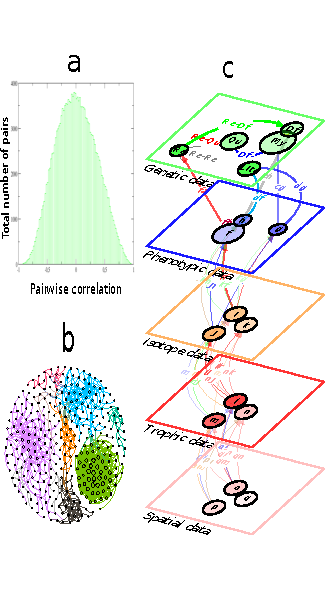
\includegraphics[width=13cm,height=14cm]{Figure3.pdf}
  \vspace{0.75 in} \hspace{-3 in}\caption{{\small Figure 3}}
\end{small}
\end{singlespace}
\end{mybox}


\begin{mybox}\begin{singlespace}
{\bf{Box 2. Deep process-based learning networks in Biodiversity research}}\\
\begin{small}
  We will implement a multilayer approach to generate process-based
  species distribution maps accounting for interdependent biological
  networks (Figure 4). Each layer will be parametrized taking
  advantage of the empirical patterns obtained from our source data
  (Box 1) and from the integration of biodiversity datasets (See
  section 4.2 Data Sources and
  $https://github.com/melian009/Robhoot/blob/master/layers/data.integration/databases.md$.)
  Most data in biodiversity are collections of small data. In areas
  such as species ranges and species interactions, there is a large
  amount of data, but only a relatively small amount of data for each
  gene, phenotype, individual or trophic interaction. To customize
  predictions accounting for interdependent biological levels it
  becomes necessary to build a formalism considering the heterogeneity
  at individual level, with its inherent uncertainties, and to couple
  these models together in a hierarchy scaling from genes, to
  phenotypes, populations, communities and species ranges, so that
  information can be borrowed from other similar levels across the
  landscape in the absence of empirical estimations. This
  individualization is becoming common in many fields
  \citep{Ghahramani:2015}. We will implement a multilayer approach
  using hierarchical Bayesian neural networks such as hierarchical
  Dirichlet processes accounting for interdependent layers (Figure 4:
  Genetic-phenotype interactions determine the interactions
  within-between species and with the abiotic environment. The final
  result of the multilayer interactions will generate a biodiversity
  distribution map for many interacting species). We will explore a
  range of topologies from bidirectional recurrent neural networks
  (BRNN) to feedforward neural networks (FNN) and reinforcement
  learning in unknown and fluctuating environments (RL)
  \citep{Schmidhuber:2015}. We will explore independent networks
  considering modularity and sparse matrices within- and
  between-layers (i.e., a highly modular pleiotropy matrix determining
  the genotype-phenotype map and a highly modular within- and
  between-species interactions with most interactions weak or zero.)
  Such scenario will produce a non-interactive species biodiversity
  map. The second scenario will take into account interactions and
  feedbacks among layers to contrast predictions between independent
  and interdependent layers in biodiversity dynamics and how the
  interactions and feedbacks alter biodiversity decline to different
  disturbance regimes \citep{Melianetal:2018}. \vspace{-3 in}
  \hspace{0.5 in}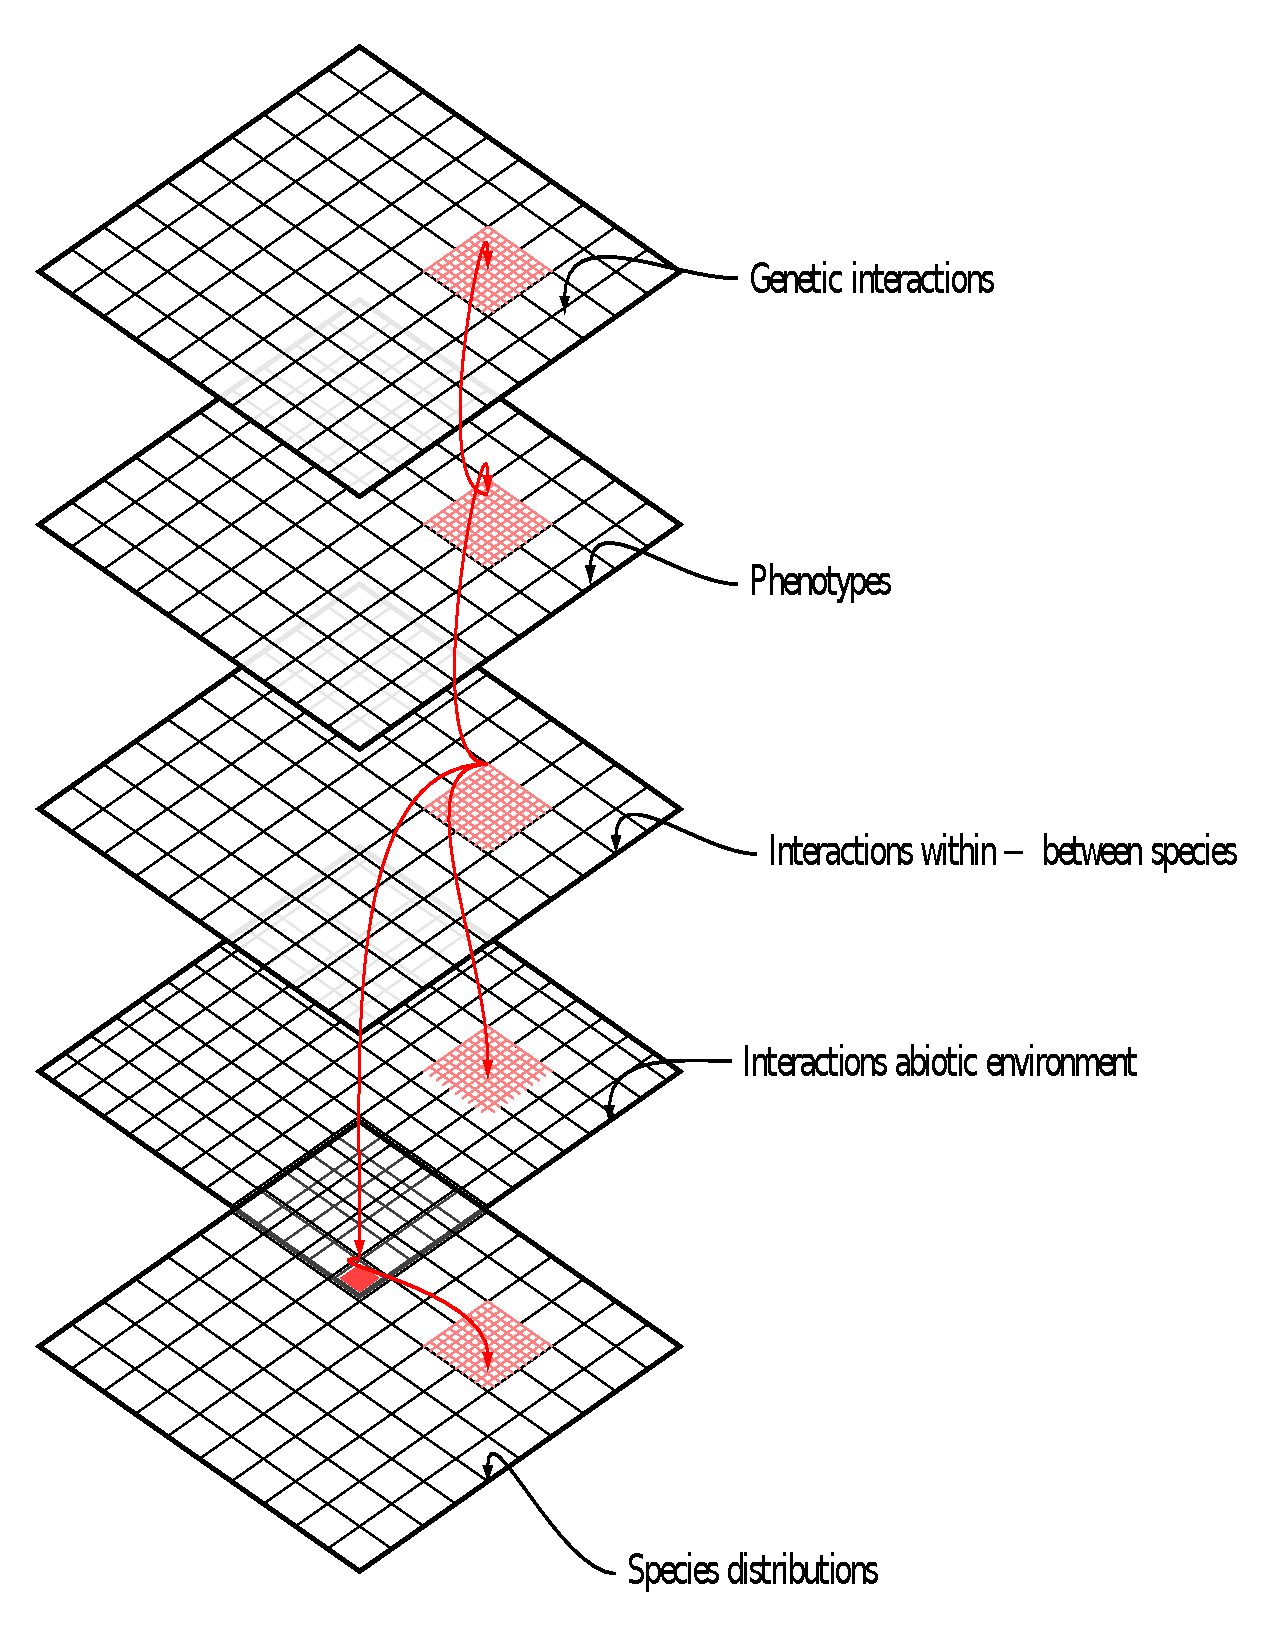
\includegraphics[width=14cm,height=10cm]{Box2b.pdf}\\
  \vspace{2 in} \hspace{0.1 in} \caption{{\small Figure 4}}
  \vspace{0.75 in}
\end{small}
\end{singlespace}
\end{mybox}

\section*{4.3 Work Packages, Milestones and Deliverables}
This project will strengthen the feedback between data-scientists and
the community of scientists in biodiversity research. This fussion
will produce two methods packages and two scientific papers. Below we
describe the timeline describing the milestones, the deliverables and
the timing to release the packages in public repositories.
\\
\\
{\bf Work packages}\\
{\bf WP1}: Data visualization\\
{\bf Lead}: SDSC, contributed data: GENOM, ECOSYS and BIOD\\
{\bf WP2}: Inference empirical patterns with our source data (Box 1 and Section 4.2)\\
{\bf Lead}: SDSC, contribution: MAIN, BIOD, CSYS, GENOME and ECOSYS\\
{\bf WP3}: Deep process-based learning networks (Box 2)\\
{\bf Lead}: SDSC, MAIN and CSYS)\\
\\
{\bf Milestones}\\
{\bf M1.1}: Uploading source data to the SDSC Platform\\
{\bf M1.2}: Visualization empirical patterns of interdependent networks\\
{\bf M2.1}: Web spidering to enrich the existing database in biiodiversity research\\
{\bf M2.2}: Animation package of the Fish collection part of the FishEc database in the
permanent exhibition hosted by the Natural History Museum in Bern\\
{\bf M3.1}: Implementation of methods for inferring patterns in interdependent networks (Box 1)\\
{\bf M3.2}: Efficient code implementation for inferring the interdependence among networks\\
{\bf M4.1}: Implementing, debugging, running and analyzing the deep process-based learning networks scenarios (Box 2)\\
{\bf M4.2}: Global biodiversity maps without and with interdependent networks\\
\\
{\bf Deliverables}\\
{\bf D1}: Data visualization package to gain insights of the interactions across biological
networks from genes to ecosystems.\\
The package will be used as highlights in a permanent exhibition of the natural
history museum in Bern. We will produce a public github repository and a
reproducible research document in Jupyter and Renku.\\
{\bf D2}: Data mining and inference patterns and processes in interdependent networks.\\
We will produce the inference package in interdependent networks. The package will
be uploaded and maintained in a github public repository. Together with the inference
package, we will produce a reproducible research document in Jupyter and Renku.\\
{\bf D3}: Scientific paper focusing on pattern inference in interdependent networks.\\
We will aim to a top general scientific journal. A reproducible research document
will be developed in github, Jupyter and Renku.\\
{\bf D4}: Scientific paper focusing on deep process-based learning networks introducing the global map of biodiversity in interdependent networks.\\
We will aim to a top general scientific journal. A reproducible research document
will be developed in github, Jupyter and Renku.

\section*{5. Requested Resources}

\subsection*{5.1 Staff}

\subsection*{5.1.1 Data science expertise}
A two years data scientist from the SDSC will be required to guarantee
the accomplishment of the word packages WP1 to WP3, and the
deliverables D1 to D4 (see Requested resources and contributed
resources below). The following are the key contributions for each
stage of the project:
\\
{\bf WP1}: Software development to complement/improve the existing
visualization and animations tools for multilayer networks. Many
libraries are rapidly emerging to integrate, analyze, and visualize
patterns in multilayer networks, yet new features
will be required to gain insights of the coupling of interacting biological networks.\\
{\bf WP2}: Machine Learning techniques to enrich the biodiversity database.\\
{\bf WP3}: Efficient code implementation to infer patterns of interactions in the empirical multilayer networks (Box 1).\\
{\bf WP4}: Analysis of the deep process-based learning networks to generate biodiversity maps accounting for interdependent networks (Box 2).\\

\subsection*{5.2 Compute and storage resources}

\subsubsection*{5.2.1 Summary}
The following are the working packages requiring computing and storage resources:\\
\\
{\bf WP1}: Run the visualizations for a small dataset containing 5-10k
individuals with genetic, phenotypic, ecological and spatial data. We
will scale the visualization for this subset to a larger dataset
containing approximately 60k fish individuals, 40k morphometric
measurements, and 8k sampling actions each containing spatial
coordinates, morphological traits, abundances, habitats and DNA
data. We expect approximately 4 GPU during 6 months (see {\bf
  SDSC{full}.{proposal}.{requested}.{resources}.{Melian}.{2019}.xlsx})
to run the visualizations and the animations using the small and the
large dataset and approx. 40 GPU servers RAM during a total period of
6-8 months.\\
{\bf WP2}: Implementing Gibbs sampling to fit the interaction
coefficients for the interactions within and between the genetic,
phenotypic, ecological and spatial data (Box 1 and 2). Our estimated
need for CPU (cores) is of 35 for a 8 months period. Please notice the
fitting for Box 1 using our source data can be quick in comparison to
the fitting to produce the biodiversity maps using deep process-based
learning networks.

We expect to be working with the following data size for our source data:
1) Data containing 5-10k individuals each containing a 20x20 gene
interaction matrix and a 40x40 phenotypic interaction matrix. The
spatial data contains 0.1k-0.5k sites each containing between 1 and 10
habitats. Each individual has coordinates within a habitat.\\
2) Data containing 50k individuals each containing a 40x40 gene
interaction matrix and a 80x80 phenotypic interaction matrix. The
spatial data contains 0.5k-1k sites each containing between 1 and 10
habitats.\\
{\bf WP3}: Implementation of the fitting in the deep process-based
learning networks (Box 2). We will be working with matrices as
described in WP2. Please notice the biodiversity maps will contain
much larger matrices because the integration between different
datasets. We expect the numbers described above will be two-three
times larger. 

\section*{5.2.2 Software packages}

The following is the list of packages and skills required to
accomplish the deliverables D1 to D4:
\\
{\bf Skill 1}: Spark GraphX to combine visualization, exploratory
analysis and computation of
metrics to infer network patterns crossing two or more networks.\\
Additional skills: Implementation of packages in python (pymnet), java (gephi), and julia (muxviz) languages.\\
\\
{\bf Skill 2}: Javascript/Jquery to enrich the biodiversity database.\\
Additional skills: Implementation of codes in python, Ruby or others to search databases.\\
\\
{\bf Skill 3}: TensorFlow. We have been working at a very preliminary
stage with a julia wrapper for TensorFlow. We are open to learn
from other packages/languanges to implement the methods required in this proposal.\\
Additional skills: Hidden random Markov fields models, Bayesian
methods (Dirichlet process among others) and deep learning networks
(bidirectional recurrent neural networks, feedforward neural networks
and reinforcement learning networks) to efficiently compute and/or
reconstruct interaction networks using genetic, phenotypic, ecological
and spatial data.

\section*{6. Contributed resources}
Dr. Victor Eguiluz, team CSYS, will join as a senior scientist during
the spring 2020 to work in the work packages WP2 (inference) and WP3
(Process-based modeling). The main task of Dr. Eguiluz will focus on:
\\
1. Implementing, debugging, running and analyzing the proposed deep
process-based learning networks scenarios (Box 2).
\\
2. Drafting scientific paper focusing on inference patterns in
interdependent networks (Deliverables D3 and D4). Please see the
document {\bf
  SDSC{full}.{proposal}.{requested}.{resources}.{Melian}.{2019}.xlsx}
for a view of the total contributed staff.
\\
Contributions for other groups:\\
{\bf MAIN}: Dr. Carlos Melian: (1 x 4)\\
Teaming up with SDSC staff and Dr. Eguiluz (0.3 x 24) to develop
pattern and process-based inference packages (Deliverables D2 to D4
with SDSC and work packages WP3 and WP4 with SDSC and Dr.
Eguiluz). \\
\\
2 months {\bf GENOM} Dr. Philine Feulner: (0.2 x 2)\\
Supervising accuracy of the genetic data included in the FishEc
dataset (WP1).
\\
2 months {\bf ECOSYS} Dr. Blake Matthews: (0.2 x 2)\\
Drafting scientific papers focusing on pattern inference and
process-based methods in interdependent networks (deliverables D3 and
D4)
\\
2 months {\bf BIOD} Prof. Ole Seehausen: (0.1 x 2)\\
Supervising accuracy of the genetic and morphological data in the
FishEc dataset (WP1)
\\
Supervision of the visualization package (D1) and organization of the
permanent exhibition of the natural history museum in Bern
\\
{\bf All the groups}\\
Drafting scientific papers focusing on pattern inference and
process-based methods in interdependent networks (deliverables D3 and
D4).


\newpage
\bibliographystyle{unsrtnat}
%\bibliographystyle{tree.bst}
\bibliography{space.bib}
\end{document}






\begin{comment}
\begin{center}
\hspace{-2 in}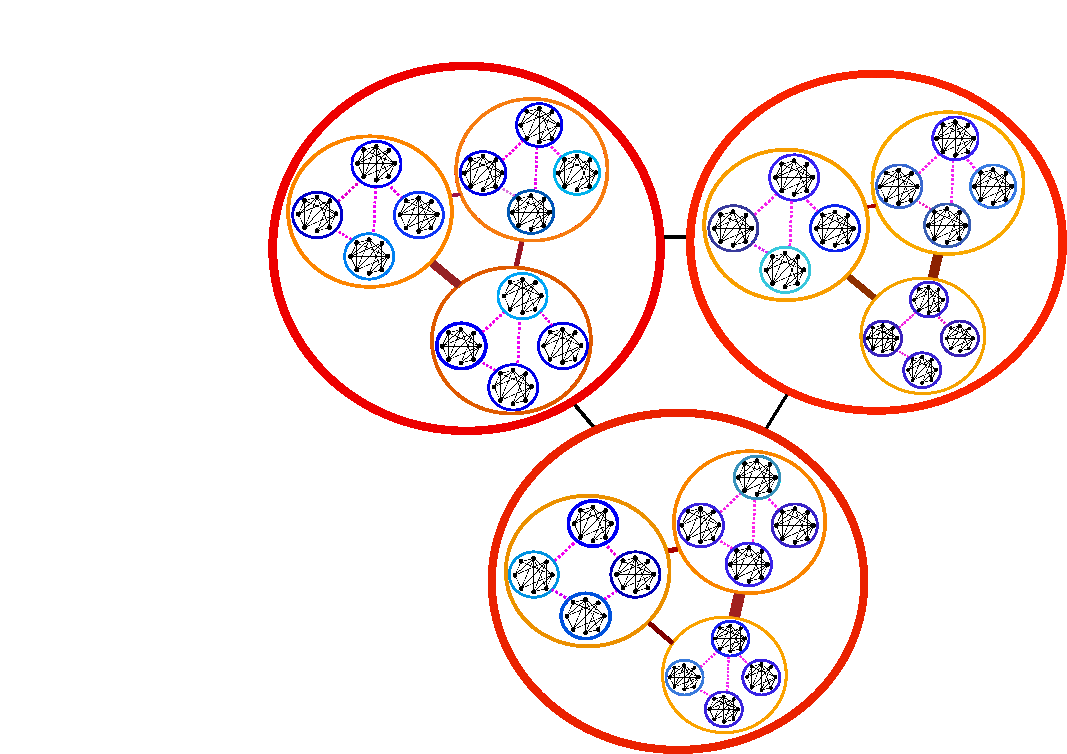
\includegraphics[width=12cm,height=9cm]{Figure1.pdf}
\\
\caption{{\small Figure 1: Hierarchical network approach: We represent a meta-ecosystem
  with patches (red), species (orange), individuals (blue), and genes
  (black). At intra-organismal level, genes interact to produce a
  trait (blue). At inter-organismal level individuals mate (dotted
  pink links) to produce the distribution of traits (blue tones). At
  population level trait distribution drives the interaction strength
  between species (brown links). The meta-ecosystem is pictured as a
  spatial network (black links) of local interaction networks.}}
\vspace{2 in}
\label{Figure 1}
\end{center}
\vspace{-1 in}
\end{comment}




\begin{comment}
To explore the interaction patterns from the
  quantitative genetic, phenotypic, ecological and spatial data we
  will use Markov Networks as an undirected graphical model to infer
  pairwise interactions for the genetic, phenotypic, ecological and
  spatial data (i.e, abundance and co-occurrence samples). To
  formulate the Markov random field of this multinomial model we
  consider that all genes, phenotypes, and species in each site $i$
  form the neighborhood of our focal species $j$, $\vec{N_{e}}_{i}$ =
  $(N_{e}_{i,1},N_{e}_{i,2},N_{e}_{i,3},...N_{e}_{i,S})^{T}$, with all
  genes, phenotypes and species potentially interacting. The
  conditional distribution, $\vec{N}_{i}$ =
  $(N_{i,1},N_{i,2},N_{i,3},...N_{i,S})^{T}$, conditioned on the
  neighborhood, $\vec{N_{e}}_{i}$ =
  $(N_{e}_{i,1},N_{e}_{i,2},N_{e}_{i,3},...N_{e}_{i,S})^{T}$ , and the
  interaction coefficients in the genetic, phenotypic and ecological
  data, $\theta$, can be based on the form of the multinomial
  probability mass function and it can be written in exponential
  family form as \citep{Mueller:2010}

\begin{align}
  f(\vec{N}_{i}|\vec{N_{e}}_{i};\theta) = exp \Bigg[\sum_{j=1}^{S-1} N_{i,j} A_{i,j}\{\vec{N_{e}}_{i}:\theta\} -  J_{i} log \left(1 + \sum_{j=1}^{S-1} exp \left[A_{i,j} \{\vec{N_{e}}_{i}:\theta\} \right] \right)\\ + log \left(\frac{J_{i}!}{N_{i,1}!...N_{i,S-1}! \ \left(J_{i} - \sum_{j=1}^{S-1} N_{i,j}\right)!}\right) \Bigg].\nonumber
\end{align}

Once the form of the parameter function,
$A_{i,j}\{\vec{N_{e}}_{i}:\theta\}$, is given, the form of $\theta$
will follow because $A_{i,j}\{\vec{N_{e}}_{i}:\theta\}$ is a function
of $\theta$. Since the Multinomial markov random field model is a
multivariate version of the Binomial model, the functional form of the
parameter function can be given by \cite{Besag:1974,Mueller:2010}
\begin{align}
A_{i,j} \{\vec{N_{e}}_{i}:\theta\} = \alpha_{i,j} + \sum_{k=1,j \neq k}^{S} \alpha_{i,j,k} N_{e}_{i,k},
\end{align}
where $\alpha_{i,j}$ is an intercept term determining the amount that
the presence of genes, phenotypes and species $j$ in site $i$ contributes to the
probabilitiy of $\vec{N}_{i}$. It directly controls the prevalence of
species $j$ in site $i$. Similarly, $\alpha_{i,j,k}$, is the
interaction coefficient defined as the amount that the co-occurrence
of species $j$ and species $k$ contributes to the probability by
determining the conditional relationship between two species in site
$i$ \cite{Harris:2016,Clarketal:2018}. Both, the intercept and the
coefficients between species are given by the community matrix
$\theta$.

We will use the Gibbs sampling function algorithm to simulate data
from the Multinomial Markov random field model. To obtain a Monte
Carlo approximation of $\theta$, based on a Gibbs sampling algorithm,
a pseudo-likelihood function might be written as
\begin{align}
  P(\theta)_{i} =  f(\vec{N}^{o}_{i}|\vec{N_{e}}_{i};\theta),
\end{align}
where $\vec{N}^{o}_{i}$ and $\vec{N_{e}}_{i}$ are the observed and
estimated neighborhood abundance vectors, respectively, and
$P(\theta)_{i}$ can be minimized using the negative log of the
pseudo-likelihood, -log($P(\theta)_{i}$)
\end{comment}




\begin{mybox}\begin{singlespace}
{\bf{Box 2. Deep process-based learning in Biodiversity research.}}\\
\begin{small} To explore the effect of evolutionary and ecological processes on multilayer networks, we propose to join deep learning with process-based networks taking into account demography, trait evolution, gene flow and selection.  1) gene interaction networks to a trait
  distribution and 2) trait distributions to interaction strength
  between species (Figure 3). The meta-ecosystem contains
  $\mathcal{P}$ patches and $\mathcal{S}$ species per patch. Gene
  interaction networks might range from traits governed by additive
  genetic variance to different network topologies taking into account
  epistasis and pleiotropy to produce a trait distribution with
  different variance for each species in each patch (Figure
  2)\citep{Stearns:2010,EyreWalker:2010,Wagner&Zhang:2011,Solovieffetal:2013,North&Beaumont:2015,Melo&Marroig:2015,Pavlicevetal:2015}.

 EQUATION 1: FITNESS IN MULTITRAIT GRAPHS
 
 EQUATION 2: TRAIT VALUE OFFSPRING


  Trait distributions obtained from additive or non-additive processes
  are then used to obtain each interaction strength extending previous
  food web models
  \citep{Loeuille&Loreau:2005,Allhoff&Drossel:2013,Melianetal:2014}. We
  generalize the function $\gamma^{t}_{ixy}$, represented as a
  Gaussian function describing the rate with which predator (or
  competitor) $y$ with trait value $z^{t}_{y}$ consumes prey (or
  competitor) $x$ with trait value $z^{t}_{x}$ in patch $i$ at time
  $t$, as
\begin{equation}
  \hspace{-0.05 in} \gamma^{t}_{ixy} =  \frac{1}{N_\alpha} \left( exp \left[ -\left(z^{t}_{y} - z^{t}_{x}\right)^2 \right] + 2\alpha \left[sgn(z^{t}_{y} - z^{t}_{x}) \left(1 - exp \left(-z^{t}_{y} - z^{t}_{x}\right)^2 \right) + sgn(\alpha) \right] \right),\hspace{-0.15 in} 
\end{equation}
where $N_\alpha$ is a normalization constant, $sgn(\mathcal{X})$ is
the sign function and $\alpha$ is the interaction selection
asymmetry. For $\alpha$ = 0, -1, and 1, predators or competitors
prefer common prey or competitors, rare prey or competitor with more
distant trait values, and rare prey or competitors with less distant
trait values, respectively. The interaction strength, $a^{t}_{ixy}$,
between species $x$ for a specific intraspecific niche width ($ianw$)
of the species $y$ in patch $i$ at time $t$ can then be approximated
as
\begin{equation}
  a^{t}_{ixy} = \int_{ianw} \gamma^{t}_{ixy} D(x)^{t} D(y)^{t} \mathrm{d}x \mathrm{d}y,
\end{equation}
where $D(x)$ and $D(y)$ are the density of the two species,
respectively.

The community matrix containing the interaction coefficients between
species $x$ and $y$ in patch $i$ at time $t$ and the connectivity
obtained from the species interspecific niche width
($ienw$)\citep{Loeuille&Loreau:2005,Allhoff&Drossel:2013} is given by
$\mathcal{A}$ = [$a^{t}_{ixy}$]. The phenotypes after interaction
selection for each prey or competition selection asymmetry scenario
and before reproduction can be used to calculate fitness using a
fitness gradient approach in the additive scenario
\citep{Guimaraesetal:2017} or without having to assume a particular
fitness function in the non-additive scenario
\citep{DeLong&Gibert:2016}. Fitness will then determine the ecological
dynamics that is represented as a spatial network of local interaction
networks.

We will run the model for many generations with each iteration
containing interaction selection, mating and migration to compute the
community matrix and the Jacobian for a gradient of dispersal values,
following the dispersal between patches $i$ and $j$, using the
dispersal matrix, $\mathcal{D}$ = [$d_{ij}$]. We will use the Jacobian
to obtain the S-map or other stability methods to study the effect of
gene interaction networks, interaction selection asymmetry, intra- and
inter-specific niche width, and dispersal dynamics on the stability of
hierarchical networks in the meta-ecosystem
\citep{Graveletal:2016,Deyletal:2017}.
 \end{small}
\end{singlespace}
\end{mybox}






\section*{4.3 Work Packages, Milestones and Deliverables}

This project will strengthen the feedback between data-scientists and the community of
scientists working with networks in ecology and evolution. This fusion will produce two
methods packages and two scientific papers. Below we describe the timeline describing the
milestones, the deliverables and the timing to release the packages in public repositories (Table
1).

CREATE TABLE LATEX

Work packages
WP1: Data visualization (Lead: SDSC, contribution data: GENOM, ECOSYS, and BIOD)
WP2: Web spidering for source data and data integration (Lead: SDSC, contribution: MAIN
and BIOD)
WP3: Data mining (Lead: SDSC and MAIN, contribution: CSYS)
WP4: Process-based modeling (Lead: SDSC, MAIN and CSYS)

FIGURE MILESTONES

Milestones
- M1.1: Uploading source data to Renga Platform
- M1.2: Visualization and animations of the source data as interdependent networks.
- M2.1: Web spidering to assist in the search of databases of the missing source data
- M2.2: Animation package of the Fish collection part of the FishEc database in the
permanent exhibition hosted by the Natural History Museum in Bern
- M3.1: Implementation of methods for inferring patterns in interdependent networks
(Box 1)
- M3.2: Efficient code implementation for inferring the interdependence among
networks
- M4.1: Implementing, debugging, running and analyzing the meta-ecosystem eco-
evolutionary network modeling scenarios (Box 2)
- M4.2: Analyzing the meta-ecosystem eco-evolutionary network modeling scenarios
parametrized using the inference patterns obtained in M3

%Table
Partner
WP
Year and Quarter
P
2019
L P
P
1
2 SDSC
SDSC GENOM
MAIN 3 SDSC MAIN CSYS M3.1
4 MAIN SDSC CSYS M4.1
1
ECOSYS BIOD M1.1
BIOD
2
M2.1
3
M1.2
4
M2.2
1
2020
2
3
4
D1
M3.2
D2 D3
M4.2 D4

Table 1


Deliverables
D1: Data visualization package to gain insights of the interactions across biological
networks from genes to metaecosystems.
The package will be used as highlights in the permanent exhibition of the natural
history museum in Bern. We will produce a public github repository and a
reproducible research document in Jupyter and Renga.
D2: Data mining and inference patterns and processes in interdependent networks
We will produce the inference package in interdependent networks. The package will
be uploaded and maintained in a github public repository. Together with the inference
package, we will produce a reproducible research document in Jupyter and Renga.
D3: Scientific paper focusing on inference patterns in interdependent networks
We will aim to a top general scientific journal. A reproducible research document
will be developed in github, Jupyter and Renga.
D4: Scientific paper focusing on process-based methods in interdependent networks
We will aim to a top general scientific journal. A reproducible research document
will be developed in github, Jupyter and Renga.

\section*{5. Requested Resources}

\section*{5.1 Staff}

\section*{5.1.1 Data science expertise}
A two years data scientist from the SDSC will be required to guarantee the accomplishment of
the word packages WP1 to WP4, and the deliverables D1 to D4
(see Requested resources and contributed resources below). The following are the key contributions for each stage of the project:

1. WP1: Software development to complement/improve the existing visualization and
animations tools for multilayer networks. Many libraries are rapidly emerging to integrate,
analyze, and visualize patterns in multilayer networks 123, yet add-hoc implementations in the
existing tools or the development of new ones will be required to gain insights of the features
of interacting biological networks.
2. WP2: Machine Learning techniques and web spidering to assist in the search of databases to
improve data integration among genetic, phenotypic, ecological and spatial data.
3. WP3: Efficient code implementation to overcome the computational challenges of inferring
patterns of interactions connecting two or more networks across the webs of life (Figure 1 and
Box 1).
4. WP4: Analysis and debugging of the process-based modeling scenarios taking advantage of
the inference patterns obtained in WP3 to decipher the mechanisms explaining the observed
patterns in the integrated datasets (Box 2).
5.2. Compute and storage resources
5.2.1. Summary
We will need data storage and computing resources for running the visualizations, and the
simulations using the data-driven inference of patterns and processes. The following are the
working packages requiring computing and storage resources:
CSWP1: Running the visualizations for a small dataset containing 5-10k individuals with
genetic, phenotypic, ecological and spatial data. We would require to scale the visualization for
this subset to a much larger dataset containing approximately 60k fish individuals, 40k
morphometric measurements, and 8k sampling actions each containing spatial coordinates,
morphological traits, abundances, habitats and DNA data. We expect the need of
approximately
4
GPU
during
6
months
(see
SDSC_full_proposal_requested_resources_Melian_2018.xlsx) to run the visualizations and the
animations using the small and the large dataset and approx. 40 GPU servers RAM during a
total period of 8 months.



CSWP3: Implementing Gibbs sampling to fit the interaction coefficients for the interactions
within and between the genetic, phenotypic, ecological and spatial data (Box 1). Our estimated
need for CPU (cores) is of 35 for a 8 months period.
We expect to be working with the following data size:
1) Data containing 5-10k individuals each containing a 20x20 gene interaction matrix and a
40x40 phenotypic interaction matrix. The spatial data contains 0.1k-0.5k sites each containing
between 1 and 10 habitats. Each individual has coordinates within a habitat.
2) Data containing 50k individuals each containing a 40x40 gene interaction matrix and a
80x80 phenotypic interaction matrix. The spatial data contains 0.5k-1k sites each containing
between 1 and 10 habitats.
CSWP4: Implementing methods to fit process-based models to the empirical patterns (Box 2).
We will be working with matrices as described in CSWP3.

\section*{5.2.2 Software packages}

The following is the list of packages and skills to accomplish the deliverables D1 to D4:
1. Main skill: Spark GraphX to combine visualization, exploratory analysis and computation of
metrics to infer network patterns crossing two or more networks.
Additional skills: Implementation of packages in python (pymnet), java (gephi), and/or
octave/julia (muxviz) languages.
2. Main skill: Javascript/Jquery to enrich the data sources proposed to be analyzed with
external databases.
Additional skills: Implementation of codes in python, Ruby or others to search databases.
3. Main skill: TensorFlow. We have been working at a very preliminary stage with a julia
wrapper for TensorFlow 4 and we are open to learn from other packages to implement the
methods required in this proposal to make them more efficient and robust.
Additional skills: Hidden random Markov fields models or Bayesian methods to efficiently
compute and/or reconstruct interaction networks using genetic, phenotypic, ecological and
spatial data.

\section*{6. Contributed resources}
Dr. Victor Eguiluz, team CSYS, will join as a senior scientist during the spring 2019 to work in
the work packages WP3 (Data mining and inference) and WP4 (Process-based modeling). The
main task of Dr. Eguiluz will focus on (Table 2):
1. Team up with the scientific staff of the SDSC to gain visualization insights of the ecological
and evolutionary processes underlying the data sources provided represented as multilayer
networks.
2. Implementing, debugging, running and analyzing the proposed meta-ecosystem eco-
evolutionary network modeling scenarios (Boxes 1 and 2).
3. Implementing linear algebra techniques to contrast the stability-diversity properties of
multilayer networks between scenarios driven by the empirical patterns and theoretical
scenarios using null or neutral models.
4. Drafting scientific paper focusing on inference patterns in interdependent networks
(Deliverables D2 and D3)
Table 1 shows the contributed resources from the staff. Please see the
SDSC_full_proposal_requested_resources_Melian_2018.xlsx document for a view of the total
contributed staff.
Table 2
CSYS Resource Type
(Researcher)
Dr. Victor Egu�luz Duration
Description of Role in the project
(in months)
100%
Drafting and implementing algorithms to
4 months
infer patterns and processes in
interdependent networks (WP3 and WP4).
Drafting scientific paper focusing on
pattern inference methods in
interdependent networks (deliverable D3)
MAIN Dr. Carlos Meli�n 30%
24 months
GENOM Dr. Philine Feulner
Partner
ECOSYS
BIOD
20%
2 months
Dr. Blake Matthews 20%
2 months
Prof. Ole Seehausen 10%
2 months
Teaming up with SDSC staff and Dr.
Egu�luz to develop pattern and process-
based inference packages (Deliverables D1
and D2 with SDSC and work packages
WP3 and WP4 with SDSC and Dr.
Egu�luz). Drafting scientific paper
focusing on process-based methods in
interdependent networks (deliverable D4)
Supervising accuracy of the genetic data
included in the FishEc dataset (WP1).
Drafting scientific papers focusing on
pattern inference and process-based
methods in interdependent networks
(deliverables D3 and D4)
Supervising accuracy of the genetic and
morphological data in the FishEc dataset
(WP1).
Supervision of the visualization package
(D1) and organization of the permanent
exhibition of the natural history museum in
Bern. Drafting scientific papers focusing
on pattern inference and process-based
methods in interdependent networks
(deliverables D3 and D4)

%\newpage
%\bibliographystyle{unsrtnat}
%\bibliographystyle{tree.bst}
%\bibliography{space.bib}
%\end{document}